% Template for PLoS
% Version 3.5 March 2018
%
% % % % % % % % % % % % % % % % % % % % % %
%
% -- IMPORTANT NOTE
%
% This template contains comments intended 
% to minimize problems and delays during our production 
% process. Please follow the template instructions
% whenever possible.
%
% % % % % % % % % % % % % % % % % % % % % % % 
%
% Once your paper is accepted for publication, 
% PLEASE REMOVE ALL TRACKED CHANGES in this file 
% and leave only the final text of your manuscript. 
% PLOS recommends the use of latexdiff to track changes during review, as this will help to maintain a clean tex file.
% Visit https://www.ctan.org/pkg/latexdiff?lang=en for info or contact us at latex@plos.org.
%
%
% There are no restrictions on package use within the LaTeX files except that 
% no packages listed in the template may be deleted.
%
% Please do not include colors or graphics in the text.
%
% The manuscript LaTeX source should be contained within a single file (do not use \input, \externaldocument, or similar commands).
%
% % % % % % % % % % % % % % % % % % % % % % %
%
% -- FIGURES AND TABLES
%
% Please include tables/figure captions directly after the paragraph where they are first cited in the text.
%
% DO NOT INCLUDE GRAPHICS IN YOUR MANUSCRIPT
% - Figures should be up\textit{loaded} separately from your manuscript file. 
% - Figures generated using LaTeX should be extracted and removed from the PDF before submission. 
% - Figures containing multiple panels/subfigures must be combined into one image file before submission.
% For figure citations, please use "Fig" instead of "Figure".
% See http://journals.plos.org/plosone/s/figures for PLOS figure guidelines.
%
% Tables should be cell-based and may not contain:
% - spacing/line breaks within cells to alter layout or alignment
% - do not nest tabular environments (no tabular environments within tabular environments)
% - no graphics or colored text (cell background color/shading OK)
% See http://journals.plos.org/plosone/s/tables for table guidelines.
%
% For tables that exceed the width of the text column, use the adjustwidth environment as illustrated in the example table in text below.
%
% % % % % % % % % % % % % % % % % % % % % % % %
%
% -- EQUATIONS, MATH SYMBOLS, SUBSCRIPTS, AND SUPERSCRIPTS
%
% IMPORTANT
% Below are a few tips to help format your equations and other special characters according to our specifications. For more tips to help reduce the possibility of formatting errors during conversion, please see our LaTeX guidelines at http://journals.plos.org/plosone/s/latex
%
% For inline equations, please be sure to include all portions of an equation in the math environment.  For example, x$^2$ is incorrect; this should be formatted as $x^2$ (or $\mathrm{x}^2$ if the romanized font is desired).
%
% Do not include text that is not math in the math environment. For example, CO2 should be written as CO\textsubscript{2} instead of CO$_2$.
%
% Please add line breaks to long display equations when possible in order to fit size of the column. 
%
% For inline equations, please do not include punctuation (commas, etc) within the math environment unless this is part of the equation.
%
% When adding superscript or subscripts outside of brackets/braces, please group using {}.  For example, change "[U(D,E,\gamma)]^2" to "{[U(D,E,\gamma)]}^2". 
%
% Do not use \cal for caligraphic font.  Instead, use \mathcal{}
%
% % % % % % % % % % % % % % % % % % % % % % % % 
%
% Please contact latex@plos.org with any questions.
%
% % % % % % % % % % % % % % % % % % % % % % % %

\documentclass[10pt,letterpaper]{article}
\usepackage[top=0.85in,left=2.75in,footskip=0.75in]{geometry}

% customized packages
\usepackage{fixltx2e}
\usepackage{stfloats}
\usepackage{subfloat}
\usepackage[caption=false,font=footnotesize]{subfig}

% amsmath and amssymb packages, useful for mathematical formulas and symbols
\usepackage{amsmath,amssymb}
% algorithm,algorithmicx,algpseudocode are used for writing pseudo code and algorithms
\usepackage{algorithm,algorithmicx,algpseudocode}
% multirow is used for adjusting the table
\usepackage{multirow}
% Use adjustwidth environment to exceed column width (see example table in text)
\usepackage{changepage}

% Use Unicode characters when possible
\usepackage[utf8x]{inputenc}

% textcomp package and marvosym package for additional characters
\usepackage{textcomp,marvosym}

% cite package, to clean up citations in the main text. Do not remove.
\usepackage{cite}

% Use nameref to cite supporting information files (see Supporting Information section for more info)
\usepackage{nameref,hyperref}

% line numbers
\usepackage[right]{lineno}

% ligatures disabled
\usepackage{microtype}
\DisableLigatures[f]{encoding = *, family = * }

% color can be used to apply background shading to table cells only
\usepackage[table]{xcolor}
\usepackage{booktabs}
% stop disconnecting vertical lines:
\setlength{\aboverulesep}{0ex}
\setlength{\belowrulesep}{0ex}
% array package and thick rules for tables
\usepackage{array}

% create "+" rule type for thick vertical lines
\newcolumntype{+}{!{\vrule width 2pt}}

% create \thickcline for thick horizontal lines of variable length
\newlength\savedwidth
\newcommand\thickcline[1]{%
	\noalign{\global\savedwidth\arrayrulewidth\global\arrayrulewidth 2pt}%
	\cline{#1}%
	\noalign{\vskip\arrayrulewidth}%
	\noalign{\global\arrayrulewidth\savedwidth}%
}

% \thickhline command for thick horizontal lines that span the table
\newcommand\thickhline{\noalign{\global\savedwidth\arrayrulewidth\global\arrayrulewidth 2pt}%
	\hline
	\noalign{\global\arrayrulewidth\savedwidth}}


% Remove comment for double spacing
%\usepackage{setspace} 
%\doublespacing

% Text layout
\raggedright
\setlength{\parindent}{0.5cm}
\textwidth 5.25in 
\textheight 8.75in

% Bold the 'Figure #' in the caption and separate it from the title/caption with a period
% Captions will be left justified
\usepackage[aboveskip=1pt,labelfont=bf,labelsep=period,justification=raggedright,singlelinecheck=off]{caption}
\renewcommand{\figurename}{Fig}

% Use the PLoS provided BiBTeX style
\bibliographystyle{plos2015}

% Remove brackets from numbering in List of References
\makeatletter
\renewcommand{\@biblabel}[1]{\quad#1.}
\makeatother



% Header and Footer with logo
\usepackage{lastpage,fancyhdr,graphicx}
\usepackage{epstopdf}
\graphicspath{{../Figures/}}
%\pagestyle{myheadings}
\pagestyle{fancy}
\fancyhf{}
%\setlength{\headheight}{27.023pt}
%\lhead{\includegraphics[width=2.0in]{PLOS-submission.eps}}
\rfoot{\thepage/\pageref{LastPage}}
\renewcommand{\headrulewidth}{0pt}
\renewcommand{\footrule}{\hrule height 2pt \vspace{2mm}}
\fancyheadoffset[L]{2.25in}
\fancyfootoffset[L]{2.25in}
\lfoot{\today}

%% Include all macros below

\newcommand{\lorem}{{\bf LOREM}}
\newcommand{\ipsum}{{\bf IPSUM}}

%% END MACROS SECTION


\begin{document}
	\vspace*{0.2in}

		{\Large\textbf\newline{{Supporting Document for Kinematics of the exoskeletons}} % Please use "sentence case" for title and headings (capitalize only the first word in a title (or heading), the first word in a subtitle (or subheading), and any proper nouns).
		}

\section*{Kinematic Modeling}
\section*{Kinematic Modeling}
The biarticular exoskeleton was designed to assist hip and knee joints. The exoskeleton has been inspired by biarticular muscles and the aim of the design was keeping the weight in proximal joint (Hip) while delivering the required power to distal joint (Knee). The parallelogram mechanism has been purposed to accomplish this goal and take advantage of biarticular muscles biological features in the exoskeleton. The purposed exoskeleton was shown in figure \ref{Fig_Exos_Kinematics_Model}\subref{Fig_Biarticular_Exo_Mechanism}.
\begin{figure*}[h!]
	\centering
	\subfloat[\small{biarticular device}]{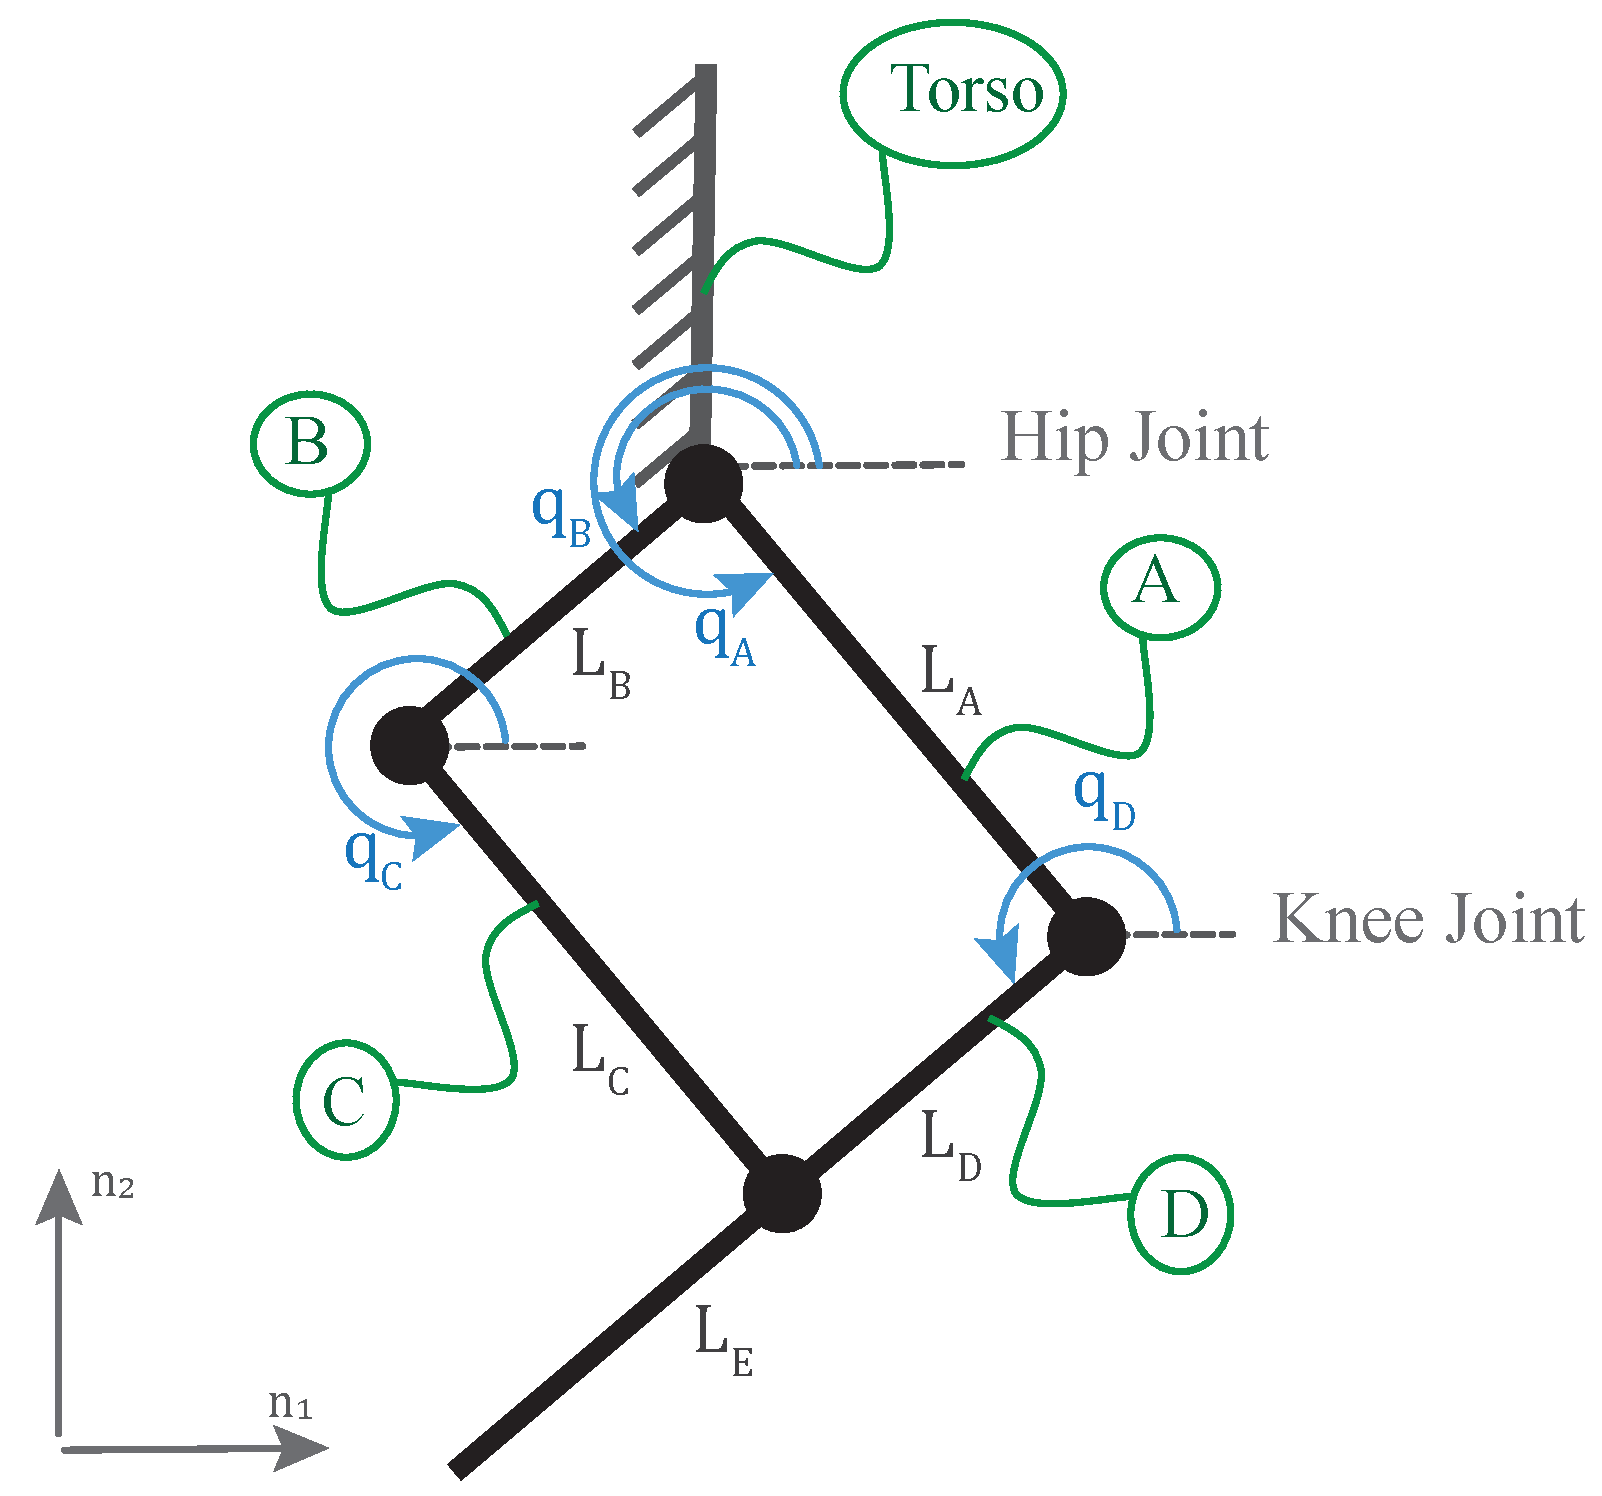
\includegraphics[width=2in]{Cartoons/Biarticular_Exo_Mechanism.pdf}
		\label{Fig_Biarticular_Exo_Mechanism}}
	\hfil
	\subfloat[\small{monoarticular device}]{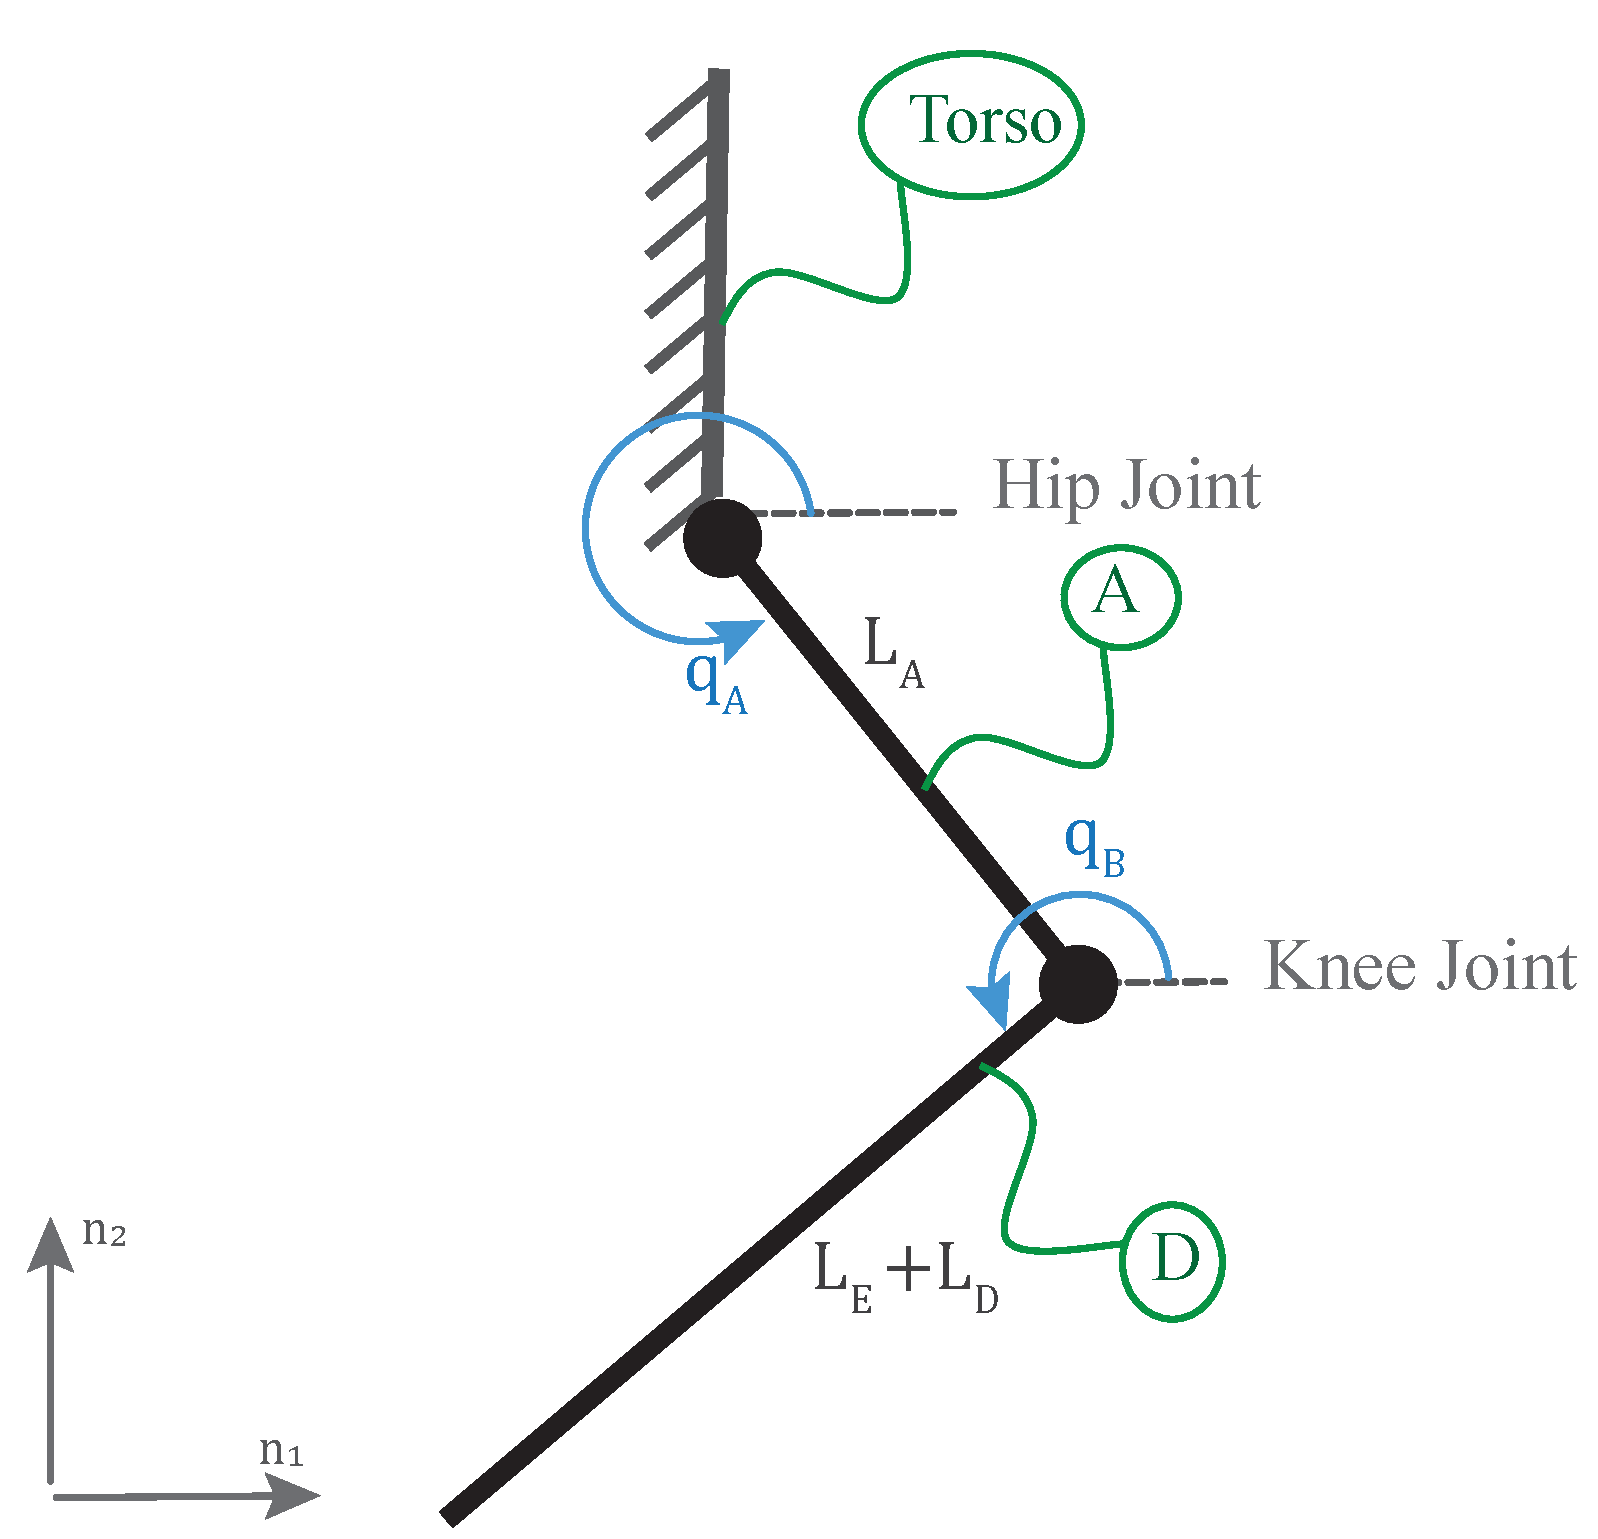
\includegraphics[width=2in]{Cartoons/Monoarticular_Exo_Mechanism.pdf}
		\label{Fig_Monoarticular_Exo_Mechanism}}
	\vspace{1mm}
	\caption{\small{\textbf{Assistive devices kinematics model.} The parallelogram mechanism has been used to model the biarticular exoskeleton and the monoarticular exoskeleton modeled by two link serial manipulator.}}
	\label{Fig_Exos_Kinematics_Model}
\end{figure*}
Where the hip joint will be assisted by applying directly the torque on the joint and second actuator torque will be applied to knee joint through the parallelogram mechanism.
\begin{align}\label{Eqn_Bi_Kin}
x_{Bi} &= l_ {A}\cos (q_ {A}) + (l_ {E} + l_ {D})\cos (q_ {B})\\
y_{Bi} &= l_ {A}\sin (q_ {A}) + (l_ {E} + l_ {D})\sin (q_ {B})
\end{align}

Monoarticular Exoskeleton can be modeled as a two-link serial manipulator as shown in figure \ref{Fig_Exos_Kinematics_Model}\subref{Fig_Monoarticular_Exo_Mechanism} where each joint is assisted by the directly joint actuator and the forward kinematics of monoarticular exoskeleton is:

\begin{align}\label{Eqn_Mono_Kin}
x_{mono} &= l_ {A}\cos (q_ {A}) + (l_ {E} + l_ {D})\cos (q_ {A} - q_ {B})\\
y_{mono} &= l_ {A}\sin (q_ {A}) + (l_ {E} + l_ {D})\sin (q_ {A} - q_ {B})
\end{align}
For both of the exoskeletons configurations the kinematics in motion level also can be easily driven and resulted Jacobian of each configurations can be written as in Eq \eqref{Eqn_Bi_Jacobian} and \eqref{Eqn_Mono_Jacobian}.

\begin{gather}\label{Eqn_Bi_Jacobian}
J_{Bi} =
\begin{bmatrix}
-l_{A}\sin{q_{A}}  & -(l_ {E} + l_ {D})\sin (q_ {B})\\
l_ {A}\cos (q_{A}) &  (l_ {E} + l_ {D})\cos (q_ {B})
\end{bmatrix}_{2 \times 2}
\end{gather}

\begin{equation}\label{Eqn_Mono_Jacobian}
\begin{aligned}
J_{Mono}&=
\left[\begin{matrix}
-l_{A}\sin{q_{A}}- (l_ {E} + l_ {D})\sin (q_ {A} - q_ {B})\\
l_{A}\cos{q_{A}} + (l_{E} + l_{D})\cos (q_{A} - q_ {B})
\end{matrix}\right.\\
&\qquad\qquad
\left.\begin{matrix}
{} (l_ {E} + l_ {D})\sin (q_ {A} - q_ {B})\\
{} - (l_ {E} + l_ {D})\cos (q_ {A} - q_ {B})
\end{matrix}\right]_{2\times 2}
\end{aligned}
\end{equation}

\end{document}
